\documentclass[11pt,xcolor=x11names,compress]{beamer}

%\usetheme{Berlin}
\usepackage{cmap}					% поиск в PDF
\usepackage{mathtext} 				% русские буквы в формулах
\usepackage[T2A]{fontenc}			% кодировка
\usepackage[utf8]{inputenc}			% кодировка исходного текста
%\usepackage[english,russian]{babel}	% локализация и переносы
\usepackage{array}
\usepackage{amsmath,amsfonts,amssymb,amsthm,mathtools} % AMS

%%% Работа с картинками
\usepackage{graphicx}  % Для вставки рисунков
%\usepackage{booktabs}% Для вставки таблиц
%%% Картинки
\usepackage{tikz} % Работа с графикой
\usetikzlibrary{decorations.fractals}
\usepackage{pgfplots}
\usepackage{pgfplotstable}
\usepackage[textfont={footnotesize}]{caption}

%% Beamer Layout %%%%%%%%%%%%%%%%%%%%%%%%%%%%%%%%%%
\useoutertheme[subsection=false,shadow]{miniframes}
\useinnertheme{default}
\usefonttheme{serif}
\usepackage{palatino}
\usepackage{color}
\usepackage{amsmath}


\definecolor{skoltechgreen}{cmyk}{0.06, 0, 0.86, 0.35}

\setbeamerfont{title like}{shape=\scshape}
\setbeamerfont{frametitle}{shape=\scshape}

\setbeamercolor*{lower separation line head}{bg=skoltechgreen} 
\setbeamercolor*{normal text}{fg=black,bg=white} 
\setbeamercolor*{alerted text}{fg=red} 
\setbeamercolor*{example text}{fg=black} 
\setbeamercolor*{structure}{fg=black} 
 
\setbeamercolor*{palette tertiary}{fg=black,bg=black!10} 
\setbeamercolor*{palette quaternary}{fg=black,bg=black!10} 

\setbeamertemplate{footline}[frame number]
\setbeamerfont{page number in head/foot}{size=\normalsize}
\setbeamertemplate{caption}{\raggedright\insertcaption\par}

\DeclareMathOperator*{\argmin}{arg\,min}
\DeclareMathOperator{\E}{\mathbb{E}}

\renewcommand{\(}{\begin{columns}}
\renewcommand{\)}{\end{columns}}
\newcommand{\<}[1]{\begin{column}{#1}}
\renewcommand{\>}{\end{column}}
%%%%%%%%%%%%%%%%%%%%%%%%%%%%%%%%%%%%%%%%%%%%%%%%%%




\captionsetup{justification=centering}
\setbeamertemplate{bibliography item}[text]
\bibliographystyle{apalike}

%\captionsetup{font=scriptsize,labelfont=scriptsize}

\title{Neural Network-based exploration of construct validity for Russian version of the 10-item Big Five Inventory}
\date{
\vspace{0.5cm}
\\
	\begin{tikzpicture}[remember picture, overlay]
     \node [inner sep=1cm] % at (6)
     {
\includegraphics[height=1cm]{Skoltech+ITMO.png}};
  \end{tikzpicture} 
	%\vspace{1cm}
	%\today
}
\author{Anastasia Sergeeva \and Bogdan Kirillov \and Alyona Dzhumagulova}
\institute{ITMO University \and Skolkovo Institute of Science and Technology}
\usepackage{graphicx}
\begin{document}

\maketitle

\begin{frame}
	\frametitle{Big Five model}
	\begin{figure}
		\centering
		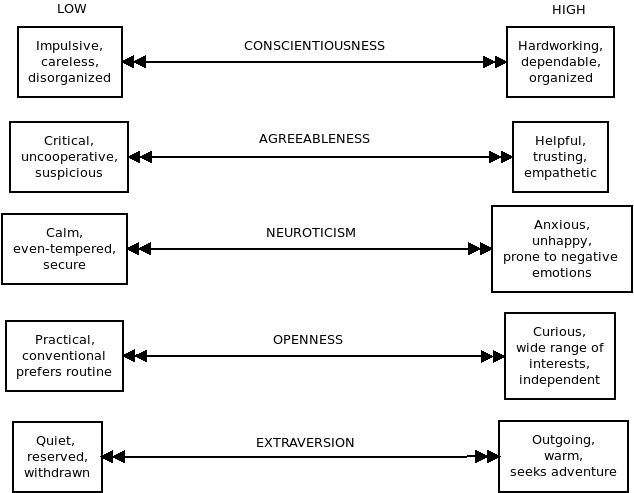
\includegraphics[width=0.7\textwidth]{Big5.png}
	\end{figure}
\end{frame}

\begin{frame}
	\frametitle{Construct validity}
	\begin{figure}
		\centering
		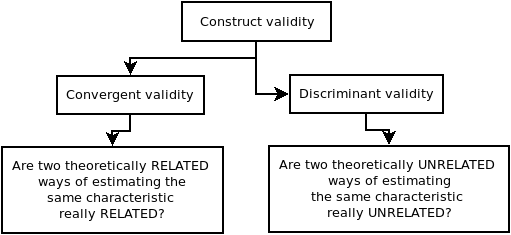
\includegraphics[width=\textwidth]{ConstructValidity.png}
	\end{figure}
\end{frame}

\begin{frame}
	\frametitle{Main contributions}
	\begin{itemize}
		\item First ever attempt to apply neural networks for construct validity evaluation;
		\item Simple qualitative approach to investigate convergent validity of questionnaire via permutation testing;
		\item Test of convergent and discriminant validity using interpretation of trained convolutional weights.
	\end{itemize}
	\centering
	The data and source code are freely available at \url{https://github.com/bakirillov/neurovalidation}.
\end{frame}

\begin{frame}
	\frametitle{Sample}
	\begin{columns}
	\begin{column}{0.5\textwidth}
	\begin{figure}
		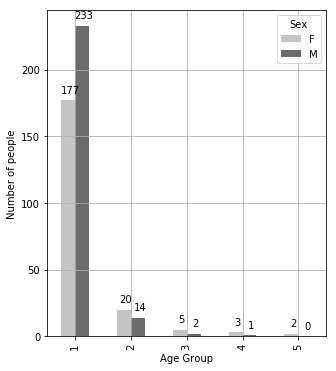
\includegraphics[width=\textwidth]{genderage.png}
	\end{figure}
	\end{column}
	\begin{column}{0.5\textwidth}
	\small
	\begin{itemize}
		\item 457 participants;
		\item 218 of them were taken from (Sergeeva et. al, 2016), available at \url{https://github.com/bakirillov/tipiru.};
		\item Age groups:
		\begin{enumerate}
			\item 10-19 years;
			\item 20-29 years;
			\item 30-39 years;
			\item 40-49 years;
			\item 50-59 years.
		\end{enumerate}
	\end{itemize}
	\end{column}
	\end{columns}
\end{frame}

\begin{frame}
	\frametitle{TIPI computation as neural network}
	\begin{columns}
	\begin{column}{0.5\textwidth}
	\scriptsize
	\begin{equation}
		E = 0.5 (TIPI_1 + reverse(TIPI_6))
	\end{equation}
	\begin{equation}
		A = 0.5 (TIPI_7 + reverse(TIPI_2))
	\end{equation}
	\begin{equation}
		C = 0.5 (TIPI_3 + reverse(TIPI_8))
	\end{equation}
	\begin{equation}
		ES = 0.5 (TIPI_9 + reverse(TIPI_4)) 
	\end{equation}
	\begin{equation}
		\label{tipi-o}
		O = 0.5 (TIPI_5 + reverse(TIPI_{10})) 
	\end{equation}
	\end{column}
	\begin{column}{0.5\textwidth}
	\begin{figure}
		\centering
		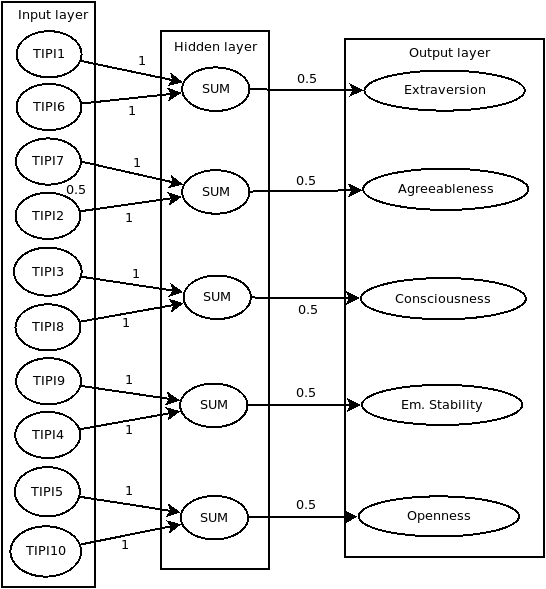
\includegraphics[width=\textwidth]{TIPIasNN.png}
	\end{figure}
	\end{column}
	\end{columns}
\end{frame}

\begin{frame}
	\frametitle{Actual network that learns TIPI-5PFQ connection}
	\begin{figure}
		\centering
		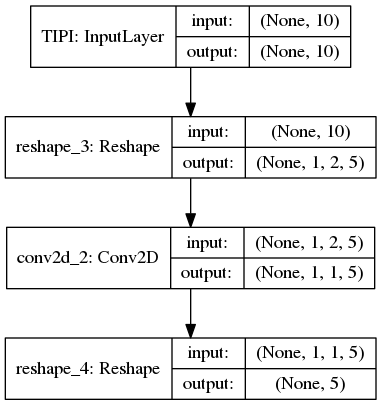
\includegraphics[width=0.6\textwidth]{tipinet.png}
	\end{figure}
\end{frame}

\begin{frame}
	\frametitle{Training behavior of the network}
	\begin{figure}
		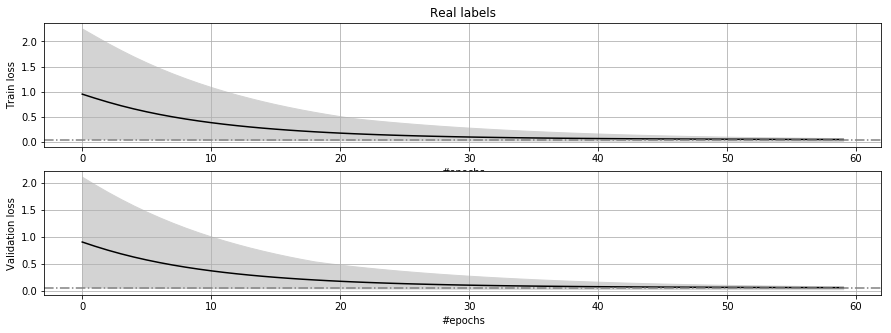
\includegraphics[width=\textwidth]{histories.png}
	\end{figure}
	\centering
	Key assumption: best possible predictions of 5PFQ that a generalizable (not overfitted) model can make from the TIPI-RU data are actually the TIPI-RU values themselves.
\end{frame}

\begin{frame}
	\frametitle{Permutation testing}
	\begin{figure}
		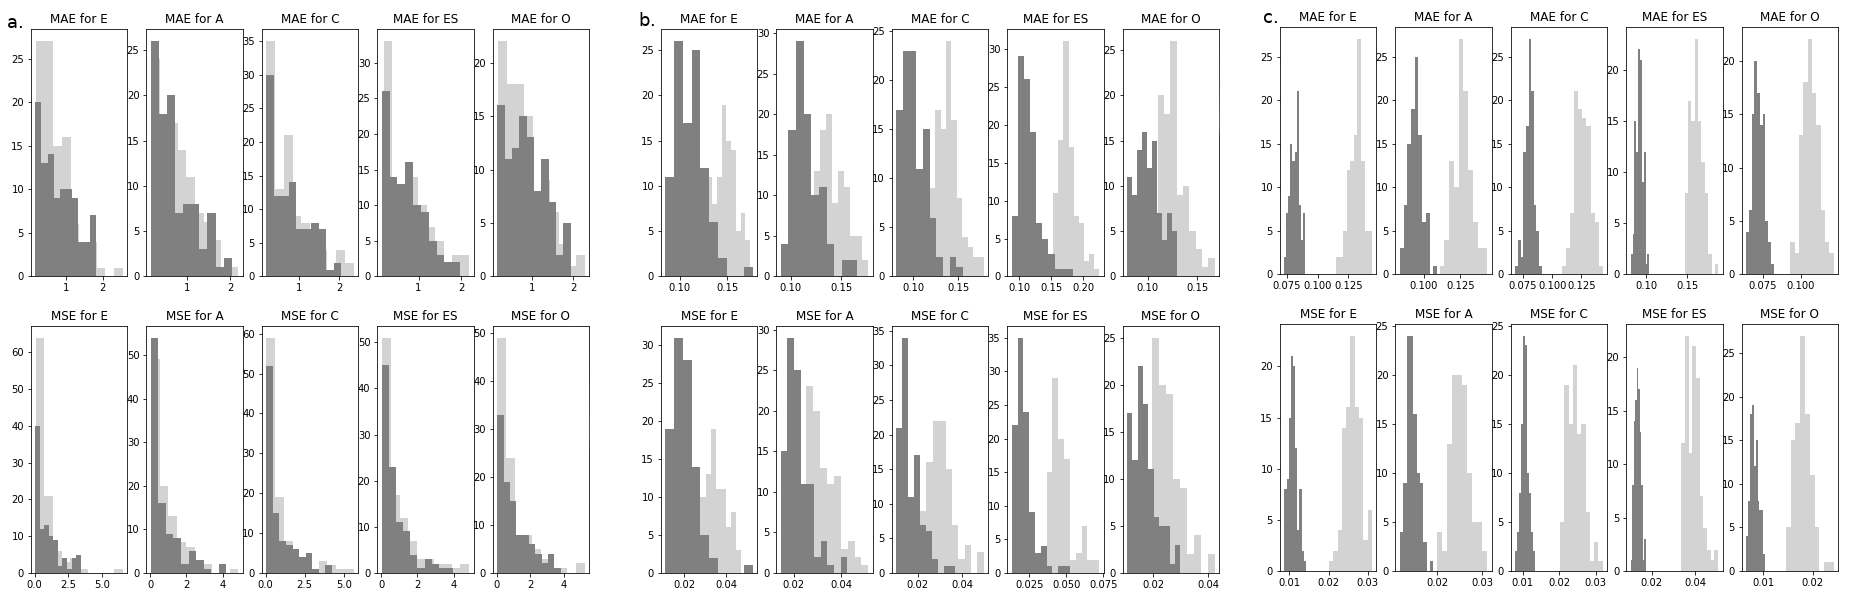
\includegraphics[width=\textwidth]{divergence.png}
	\end{figure}
	\centering
	Divergence of two distributions shows presence of learnable connection between TIPI-RU and 5PFQ.
\end{frame}

\begin{frame}
	\frametitle{Kolmogorov-Smirnov test}
	\begin{figure}
		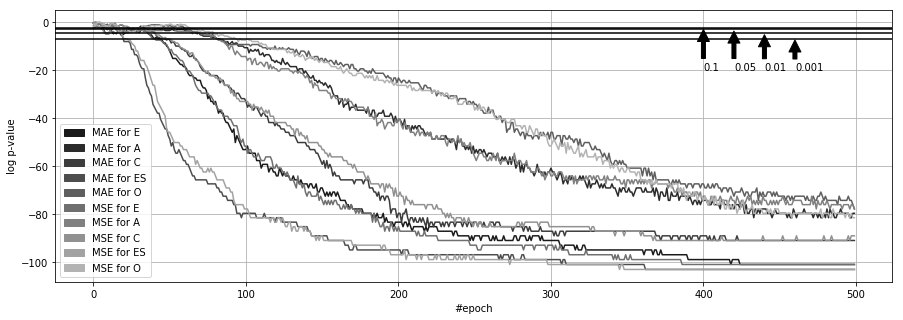
\includegraphics[width=\textwidth]{pvalues.png}
	\end{figure}
	\centering
	KS-test converges with the graphical comparison: the p-values go down during the training.
\end{frame}

\begin{frame}
	\frametitle{Interpretation of trained weights}
	\begin{figure}
		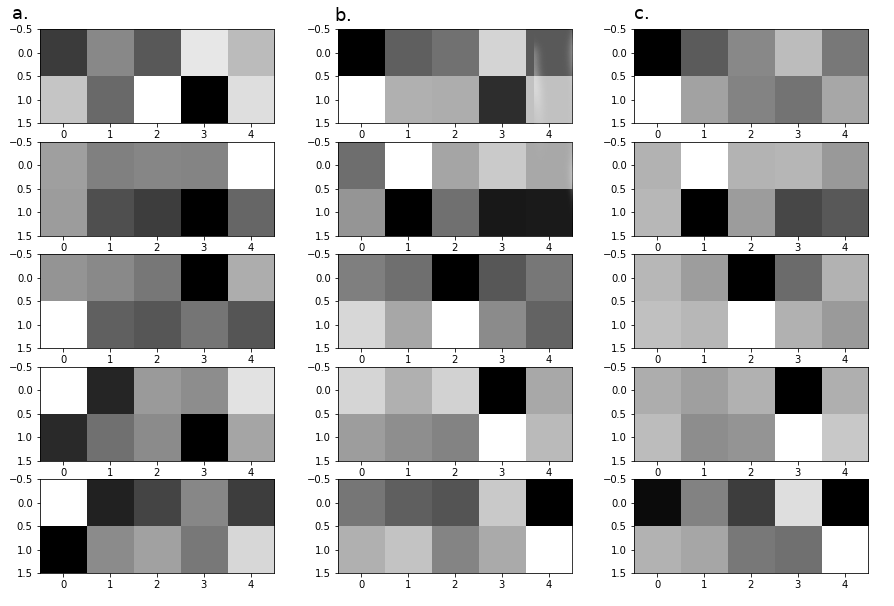
\includegraphics[width=0.75\textwidth]{interpretation.png}
	\end{figure}
	\centering
	Visualized convolutional weights mimic structure of data. Sign reversal in Agreableness is captured. Openness is inconsistent.
\end{frame}

%\begin{frame}
%	\frametitle{Future studies}
%	\begin{itemize}
%		\item Generalization of the pipeline for any questionnaire;
%		\item Further investigation of connection amongs various psychological models via NNs.
%	\end{itemize}
%\end{frame}

\begin{frame}
	\frametitle{Contact information}
	\begin{columns}
	\begin{column}{0.33\textwidth}
		\small
		\begin{figure}
			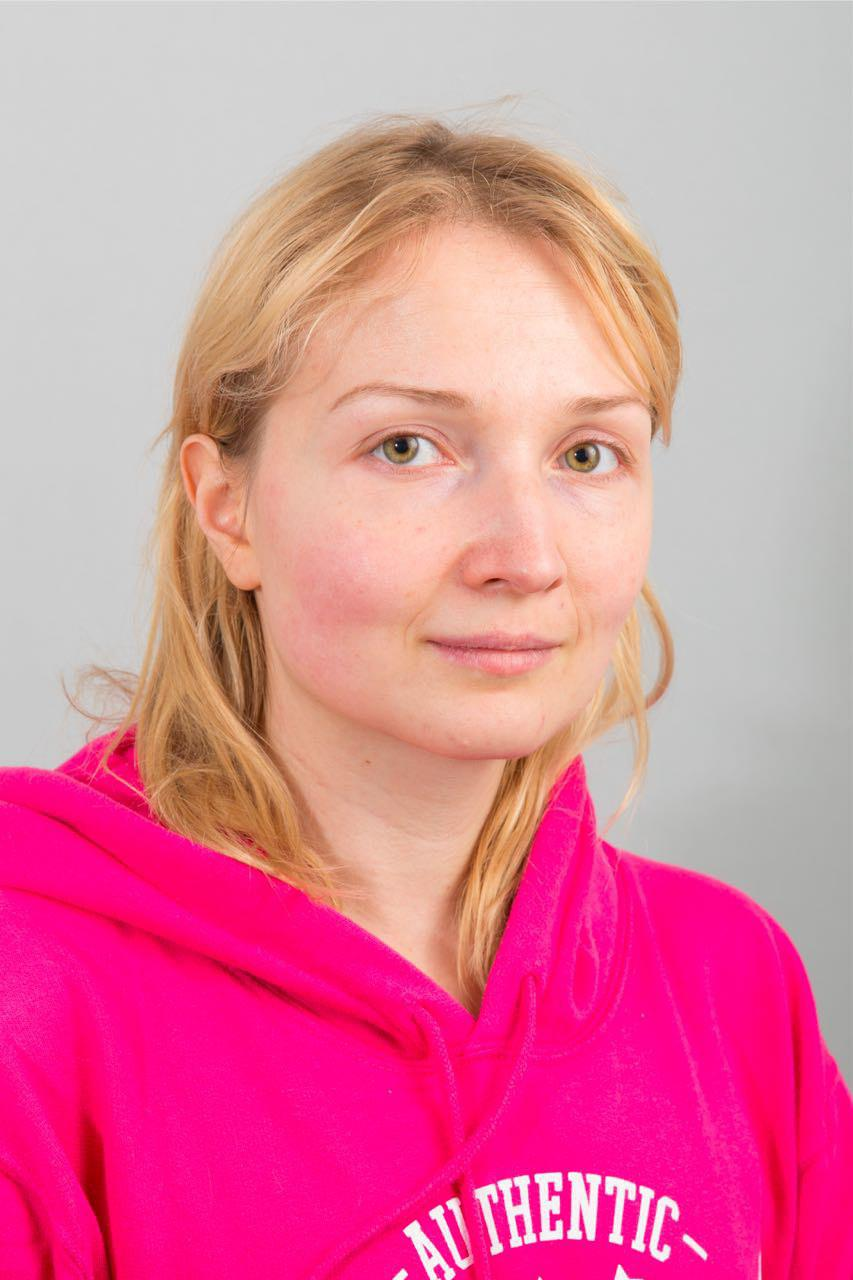
\includegraphics[width=0.8\textwidth]{Asya.png}
		\end{figure}
		\centering
		Anastasia Sergeeva \newline
		\url{an.se.sergeeva@gmail.com}
	\end{column}
	\begin{column}{0.33\textwidth}
		\small
		\begin{figure}
			
\includegraphics[width=\textwidth]{Bogdan.jpg}
		\end{figure}
		\centering
		Bogdan Kirillov \newline
		\url{Bogdan.Kirillov@skoltech.ru}
	\end{column}
	\begin{column}{0.33\textwidth}
		\small
		\begin{figure}
			
\includegraphics[width=\textwidth]{Alyona.jpg}
		\end{figure}
		\centering
		Alyona Dzhumagulova \newline
		\url{aledjuna@gmail.com}
	\end{column}
	\end{columns}
\end{frame}

\end{document}